\chapter{Related Work}

\section{Autonomous Driving}

\section{Roundabouts in Law}
% In Deutschland gibt es kein Gesetzt was den genauen Konstuktion von Kreisverkehren vorschreibt.
% Stattdessen werden die Elemente der Landstraßen und Stadtstraßen in Richtlinien für die Anlage von Landstraßen (RAL) bzw.
% den Richtlinien für die Anlage von Stadtstraßen (RASt) behandelt. Diese Richtlinien sind auch für die
% Wahl einer zweckmäßigen Knotenpunktart bei der Verknüpfung von Straßen maßgebend. Für diese Abreit sind die 
% Richtlinien für die Anlage von Stadtstraßen (RASt) relevant. Die dort behandelten Abwägungsüberlegungen orientieren sich an verkehrlichen Größen, umfeldbezogenen Merkmalen,
% wirtschaftlichen Kriterien und raumordnerischen oder städtebaulichen Vorgaben. Die Richtlinien regeln auch grundlegend die entwurfstechnische und betriebliche Ausbildung von Kreisverkehren.
%
In Germany, there is no law stipulating the exact construction of roundabouts.
Instead, the elements of the rural roads and city streets are dealt with in Directives for the Design of rural roads \cite{ral13}
and the Directives for the Design of Urban Roads \cite{rast06}. These guidelines are also relevant to the choice of a convenient junction type when linking roads.
The considerations discussed there are based on traffic variables, area-related characteristics, economic criteria and spatial planning or urban planning requirements. 
The guidelines also regulate the basic design and operational formation of roundabouts.
The  Directives for the Design of Urban Roads \cite{rast06} are relevant for this dispute. Since the access the RASt ist limited, most of the information is coming from
\cite{man06} whereupon RASt is based on.
\subsection{Elements of a Roundabout}

\begin{figure}[!ht]
%%\begin{center}
\caption{Definition of individual design elements and dimensions of a roundabout \cite{man06}}
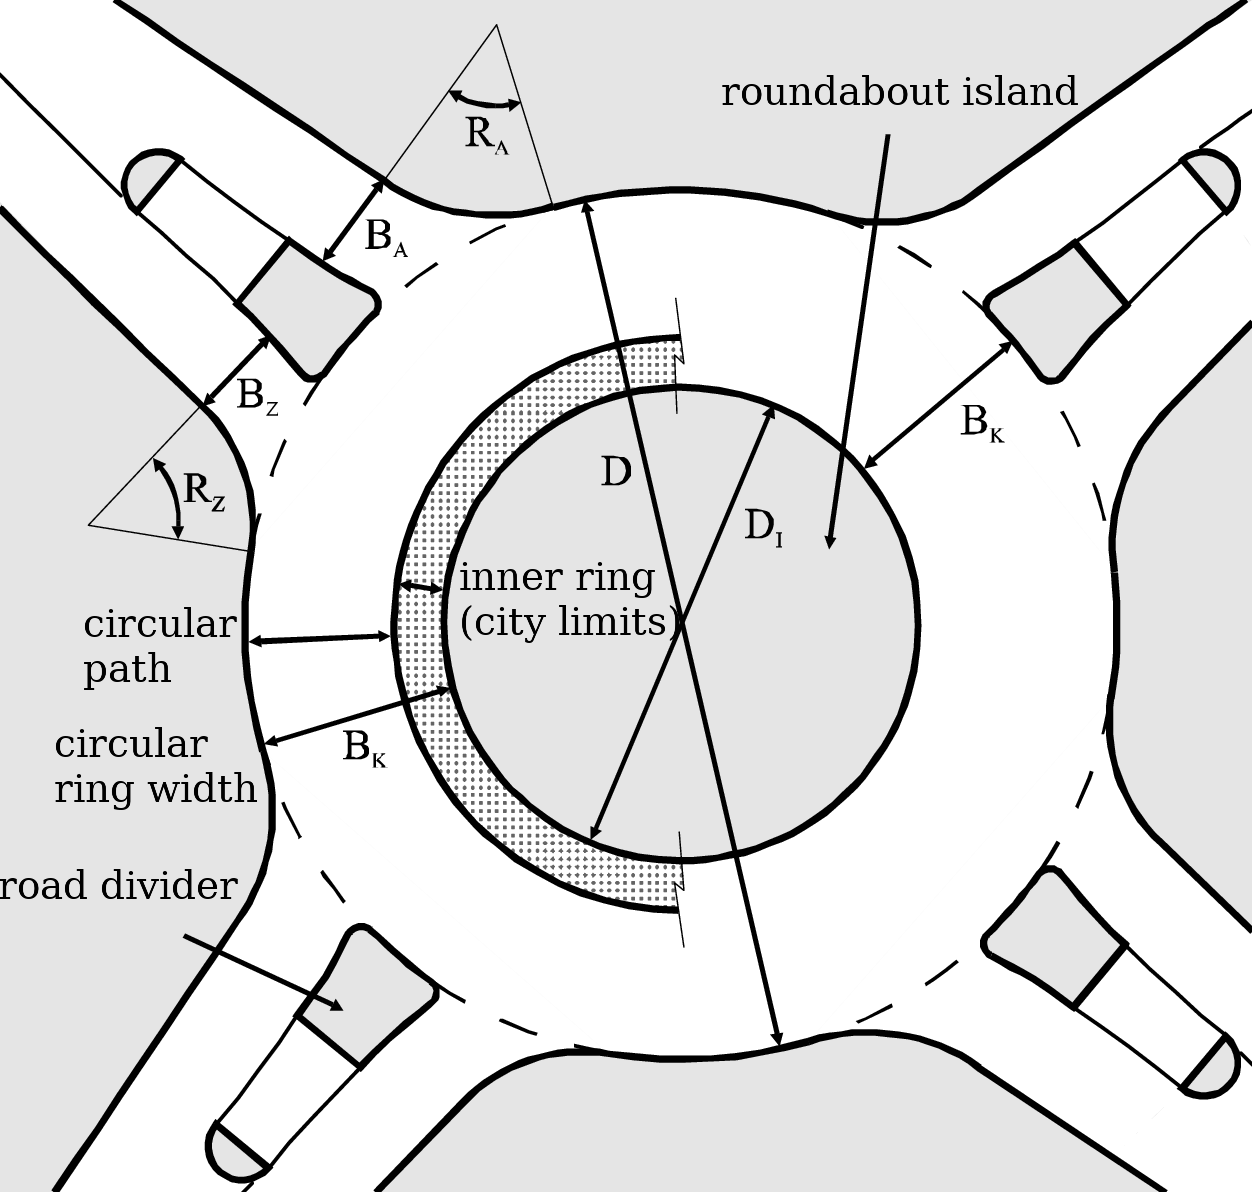
\includegraphics[width=0.7\textwidth]{bilder/kreisverkehr.png} %70% der Textbreite
\label{roundabout_parts}
%%\end{center}
\end{figure}


\begin{defi}[roundabout island]
The roundabout island is the constructional area in the middle of the roundabout, which is surrounded by vehicles.
For miniature roundabouts, the roundabout island is crossable. \cite{man06}
\end{defi}

\begin{defi}[circular path]
%Die Kreisfahrbahn ist die Fahrbahn, die zum Umfahren der Kreisinsel
%dient. Ein ggf. vorhandener Innenring ist verkehrsrechtlich nicht Be-
%standteil der Kreisfahrbahn (VwV-StVO zu §9a V., Rn. 5).

%%TODO
The circular path is the road that serves to drive the roundabout island. An inner ring, if present, is not part of the circular path (VwV-StVO zu §9a V., Rn. 5). \cite{man06}
\end{defi}

\begin{defi}[circular ring with ($B_K$)]
% Die bauliche Breite umfasst die Kreisfahrbahn und einen ggf. gepflasterten
% Innenring. Sie ist abhängig vom Außendurchmesser und der angestrebten
% Verkehrsführung (ein- oder zweistreifig). Die Randstreifenbreite orientiert
% sich an der maßgebenden durchgehenden Fahrbahn.
The structural width includes the circular track and a paved inner ring, if any. It is dependent on the outer diameter and the desired traffic routeing (one or two lanes). 
The edge strip width is oriented on the relevant continuous roadway. \cite{man06}
\end{defi}

\begin{defi}[outer diameter ($D$)]
The outer diameter is measured at the outer edge of the circular ring. It is the essential measure for describing the size of the roundabout. \cite{man06}
\end{defi}

\begin{defi}[inner diameter ($D_I$)]
The inner diameter is the diameter of the roundabout island. \cite{man06}
\end{defi}

\begin{defi}[road divider]
% Der Fahrbahnteiler ist die baulich ausgeführte Insel zwischen Kreisausfahrt
% und -zufahrt einer angeschlossenen Straße. Er dient der Trennung der
% Kreisaus- und -zufahrten, der Führung des Verkehrs sowie den Fußgängern
% und Radfahrern als Überquerungshilfe.
%
The road divider is the structurally designed island between the circular exit
and circular driveway. It serves to separate the circular exit and circular driveway, the management of the traffic, as well as the pedestrians and cyclists as cross-bordering aid. \cite{man06}
\end{defi}

\begin{defi}[lane width of the circular driveway ($B_Z$) and circular exit ($B_A$)]
% Die Breite der Kreiszufahrt und Ausfahrt wird am Beginn der Eckausrundung gemessen.
The width of the circular driveway and exit is measured at the beginning of the corner. \cite{man06}
\end{defi}

\begin{defi}[Corner rounding radius ($R_Z$ and $R_A$) ]
% Dies ist der Radius der Ausrundung am rechten Fahrbahnrand zwischen 
% der Kreiszufahrt und der Kreisfahrbahn. Bei einem Korbbogen mit einer
% Radienfolge aus drei unterschiedlichen Radien ist RZ der Radius R2 des
% mittleren Bogens. Bei der Ausbildung des Fahrbahnrandes als Schleppkurve ist RZ der kleinste Radius des Fahrbahnrandes.
% 
This is the radius of the rounding at the right edge of the road between the circular driveway and the circular path.
For a elliptical arch with a radius sequence of three different radii, $R_Z$ is the radius $R_2$ of the central arc.
When the road edge is formed as a tractrix, $R_Z$ is the smallest radius of the road edge. \cite{man06}
\end{defi}

\subsection{Types of Roundabouts}
There are several types of roundabouts, which are differentiated by the different application criteria and the partly different design principles according to the situation inside and outside built areas.
Furthermore, a division is made as a function of its size. \cite{man06}


\subsubsection{Mini Roundabout}

\begin{figure}[!ht]
%\begin{center}
\caption{Mini Roundabout \cite{man06}}
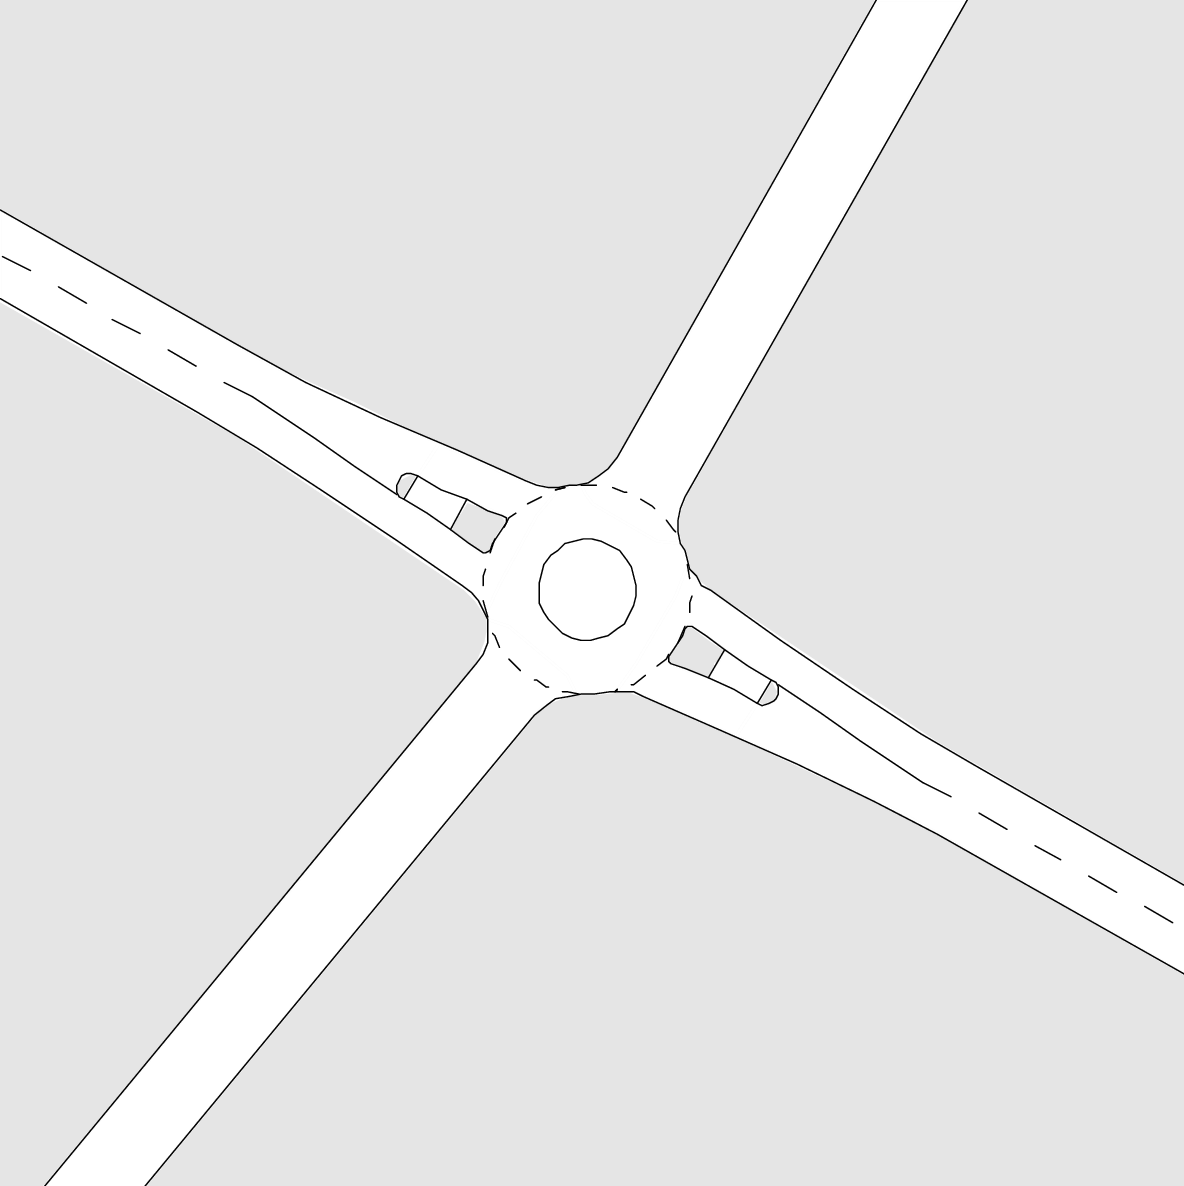
\includegraphics[width=0.5\textwidth]{bilder/mini_roundabout.png} %70% der Textbreite
\label{roundabout_mini}
%\end{center}
\end{figure}

Within built-up areas, smaller outer diameters are possible under certain conditions.
These roundabouts are called mini roundabout. The roundabout island must then be capable of being passed over.
The outer diameter should be at least 13 m, so that the circular island does not become too small.
Larger outer diameters make driving easier. Outer diameters of more than 22m, however, do not offer any transport advantages.
From an outside diameter of about 22 m, therefore, the installation of a small roundabout with 26 m is generally more convenient.
Bypasses are generally not required in the areas where mini roundabout can be used.


\subsubsection{Small Roundabout}

\begin{figure}[!ht]
%\begin{center}
\caption{Small Roundabout \cite{man06}}
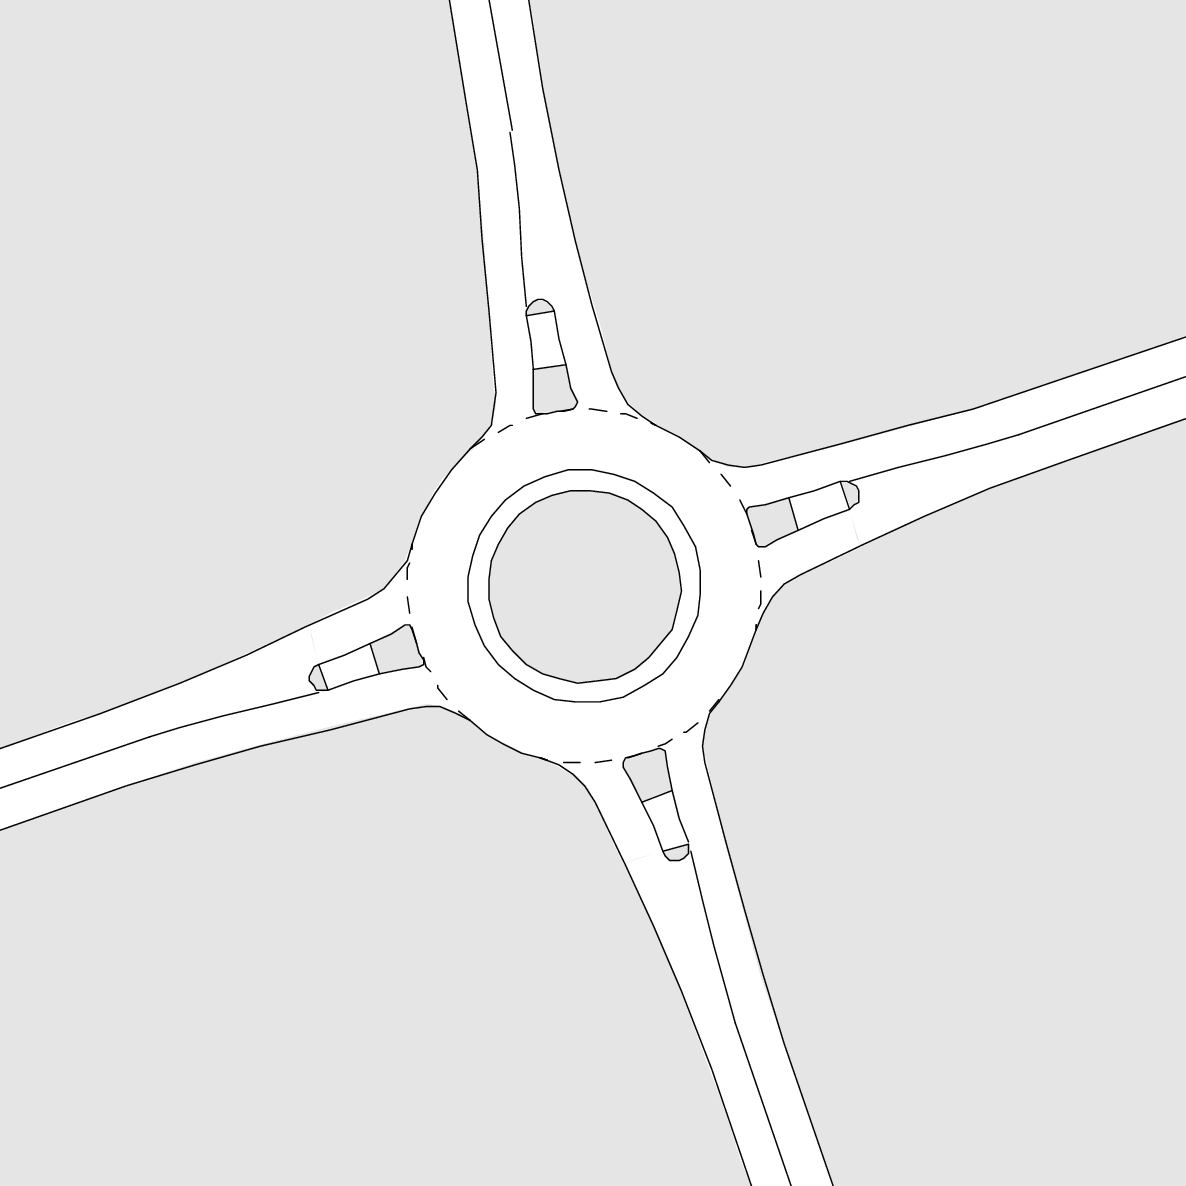
\includegraphics[width=0.5\textwidth]{bilder/small_roundabout.png} %70% der Textbreite
\label{roundabout_small}
%\end{center}
\end{figure}

The small roundabout has a single lane circular path and single lane circular driveways and exits. The roundabout island is not passable.
The outer diameter must be at least 26 m. Bypasses can be set up for driving geometric reasons or to increase performance.


\subsubsection{Two-lane Passable Roundabout}

\begin{figure}[!ht]
%\begin{center}
\caption{Two-lane Passable Roundabout \cite{man06}}
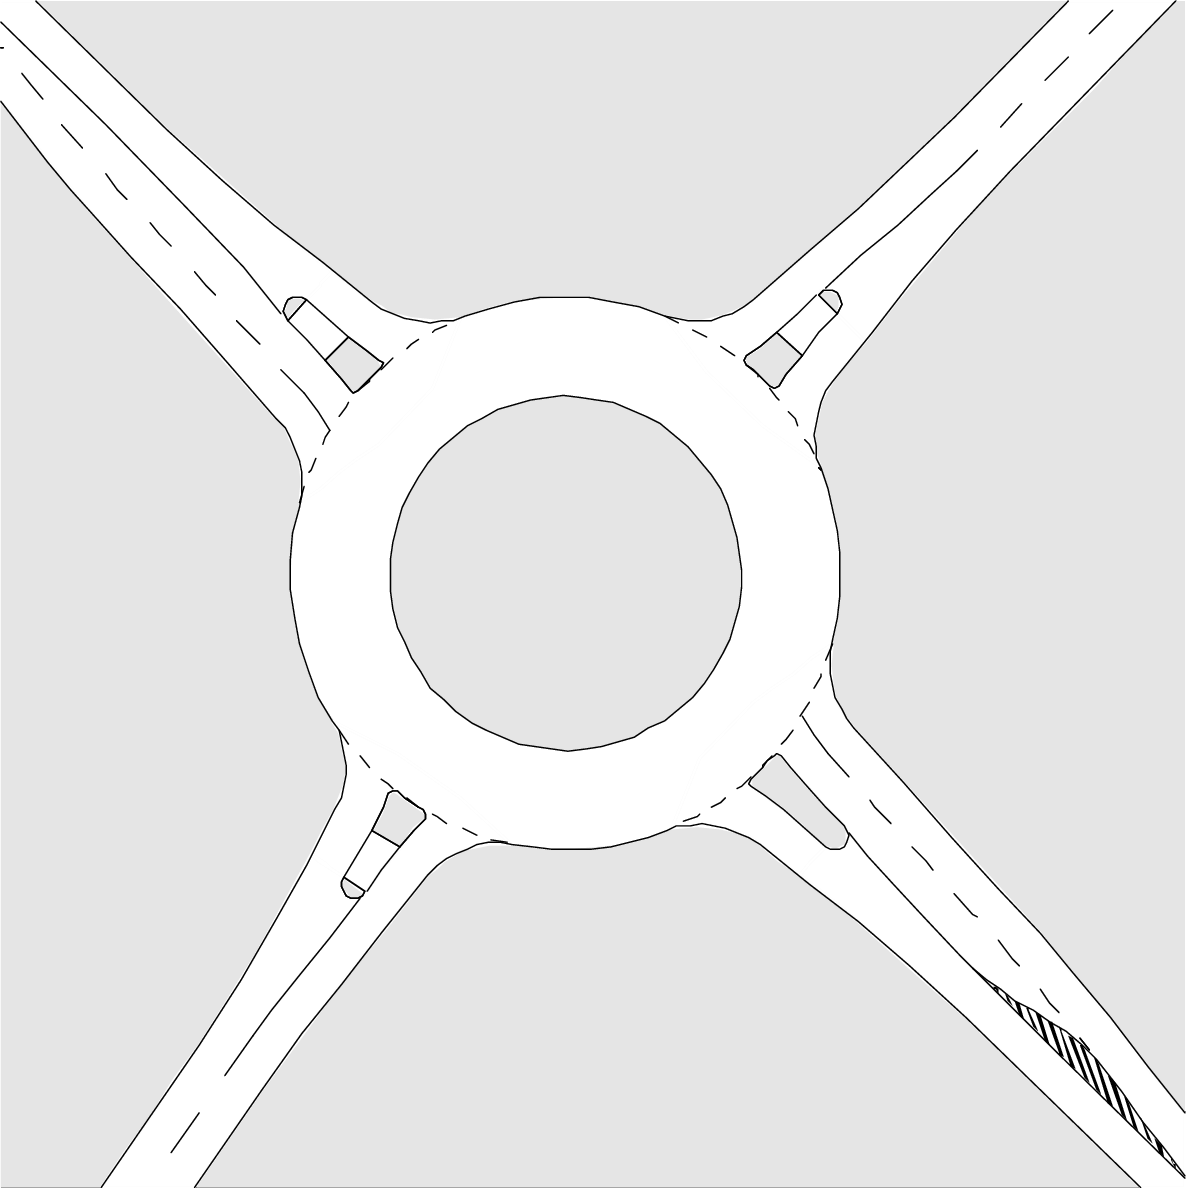
\includegraphics[width=0.5\textwidth]{bilder/twolaned_roundabout.png} %70% der Textbreite
\label{roundabout_twolaned}
%\end{center}
\end{figure}

% Reicht die Kapazität des Kleinen Kreisverkehrs nicht aus und kann diese nicht durch die Anlage von Bypässen sicher gestellt werden,
% kann die Kreisfahrbahn eines Kleinen Kreisverkehrs zweistreifig befahrbar ausgebildet werden.
% An einem solchen Kreisverkehr ist die Kreisfahrbahn so breit, dass Pkw im Kreis nebeneinander fahren können.
% Wird eine weitere Erhöhung der Kapazität erforderlich, können einzelne Kreiszufahrten ebenfalls zweistreifig ausgeführt werden,
% wenn Fußgänger und Radfahrer regelmäßig nicht zu berücksichtigen sind. Kreisausfahrten werden aus Sicherheitsgründen immer einstreifig ausgeführt.
% Aus geometrischen Gründen muss der Außendurchmesser bei zweistreifiger Befahrbarkeit mindestens 40 m betragen.
%
If the capacity of the small roundabout is not sufficient and can not be ensured by the installation of bypasses,
the circular path of a small roundabout can be designed to be two-lane driveable.
At such a roundabout, the circular path is so wide that cars can travel side by side in a circle.
If a further increase in the capacity is required, individual circular driveway can also be carried out in two lanes, if pedestrians and cyclists are not to be considered regularly.
For safety reasons, circular exits are always carried out in single lanes.
For geometrical reasons, the outer diameter must be at least 40 m for two-laned accessibility.


\subsubsection{Large Roundabout}


\begin{figure}[!ht]
%\begin{center}
\caption{Large Roundabout \cite{man06}}
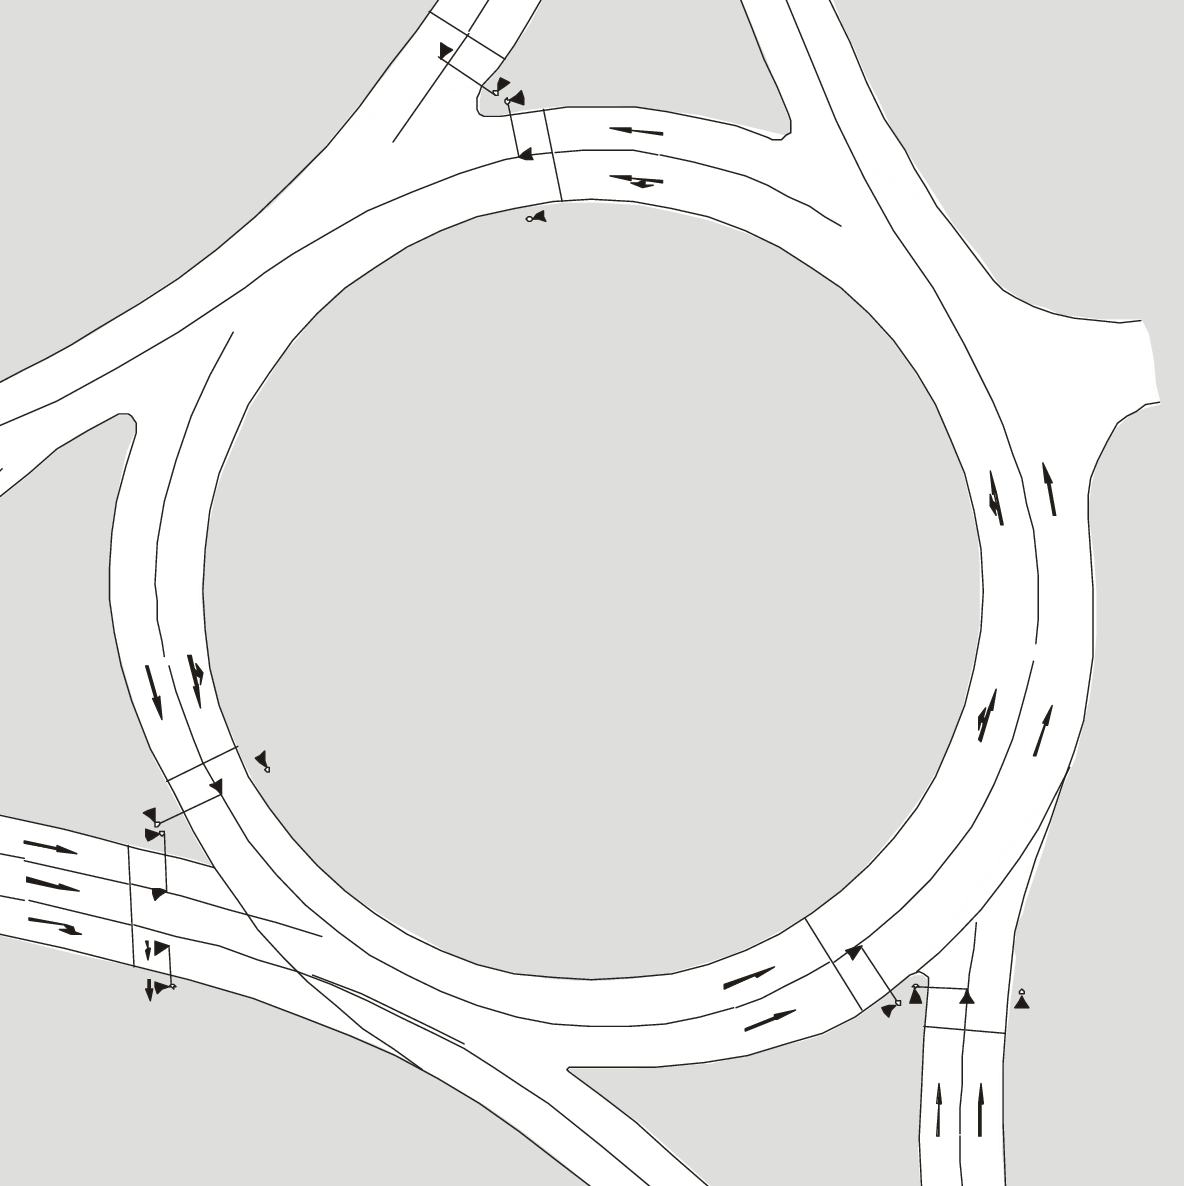
\includegraphics[width=0.5\textwidth]{bilder/large_roundabout.png} %70% der Textbreite
\label{roundabout_large}
%\end{center}
\end{figure}

%Große Kreisverkehre mit zwei oder mehreren durch Markierungen gekennzeichnete Fahrstreifen auf der Kreisfahrbahn sollen bei enger
%Abstimmung zwischen Knotenpunktentwurf und Verkehrssteuerung nur mit Lichtsignalanlage betrieben wer den.
Large Roundabouts with two or more lanes marked by markers on the circular path should be operated with a light signaling system only,
if the nodal point design and traffic control are closely coordinated.


\section{Middleware OpenDAVINCI}
Autonome Software ist typischer weise ein verteiletes System, auf heutigen Fahrzeugen basiert dieses System auf ECUs und Bussystemen wie CAN,LIN.
Verteilete Sysoftware vereinfacht es komplexe Komponenten innheralb des Systems zu integreieren. Im bereich des Autonomen Fahrens iust der Historische aufbau von Fahrzeugen
mit ECU'S und can jedoch nicht optimal. Um die vielen benötigekten Komponenten zu handhaben, ist es von vorteil Komponenten auch innerhalb eines ECU's bzw einer Recheneinheit
zu entkoppeln. Für diesen Zweck gibt es beireits mehrer middelwares die unteranderm die Kommunikation innerhalb der Komponenten handhaben und abstrahieren.
m Rahmen des Copplar Projekets, wird hier die OpenDaVINCI middleware genutzt. OpenDaVINCI ist eine echtzeitfähige laufzeitumgebeung konzipiert für Autonome Fahrzeuge.
OpenDaVINCI basiert auf Hesperia \cite{Berger2010}. Die Kommunikation zwischen den Komponenten basiert in OpenDaVINCI UDP Multicast, welches eine Echtzeitfähige Kommunikation zwischen
den Komponenten Ermöglicht \cite{Kurose2013}. Für die Kommunikation bietet OpenDaVINCI Time-triggered sender und Data-triggered receiver an, von welchem in folgenden der Data-triggered receiver
für die Anbindung der Software genutzt wird. Weiterhin bietet OpenDaVINCI viele weiter Funktionalitäten die das Handling von World Geodetic System 1984 (WGS84) Korridinaten an, welches für die Umwandlung
von GPS koordinaten in lokale kartesische genutzt werden kann. Dazu ist die Angabe einer referenz GPS postion nötig, welche um den Berechnugsfehler klein zu halten,
nicht zu weit entfernt sein sollte.


\section{Test Platform}
Die in dieser Abreit genutze Testplatform ist ein Volvo XC90 (2015) SUV. Dies Testpaltform ist mit vielen Sensoren zur Umfeldwarnehmung ausgestattet.
Dazu zählen fünf Radar Sensoren, rund um das Fahrzeug. Wobei das Front Radar über eine Größere Reichweite verfügt. Sowie eine
Stereo Kamera und ein Velodyne VLP-16 LiDAR. Die Anordnung der Sensoren kann \cref{platform} entnommen werden.


\begin{figure}[!ht]
%\begin{center}
\caption{Test Platform}
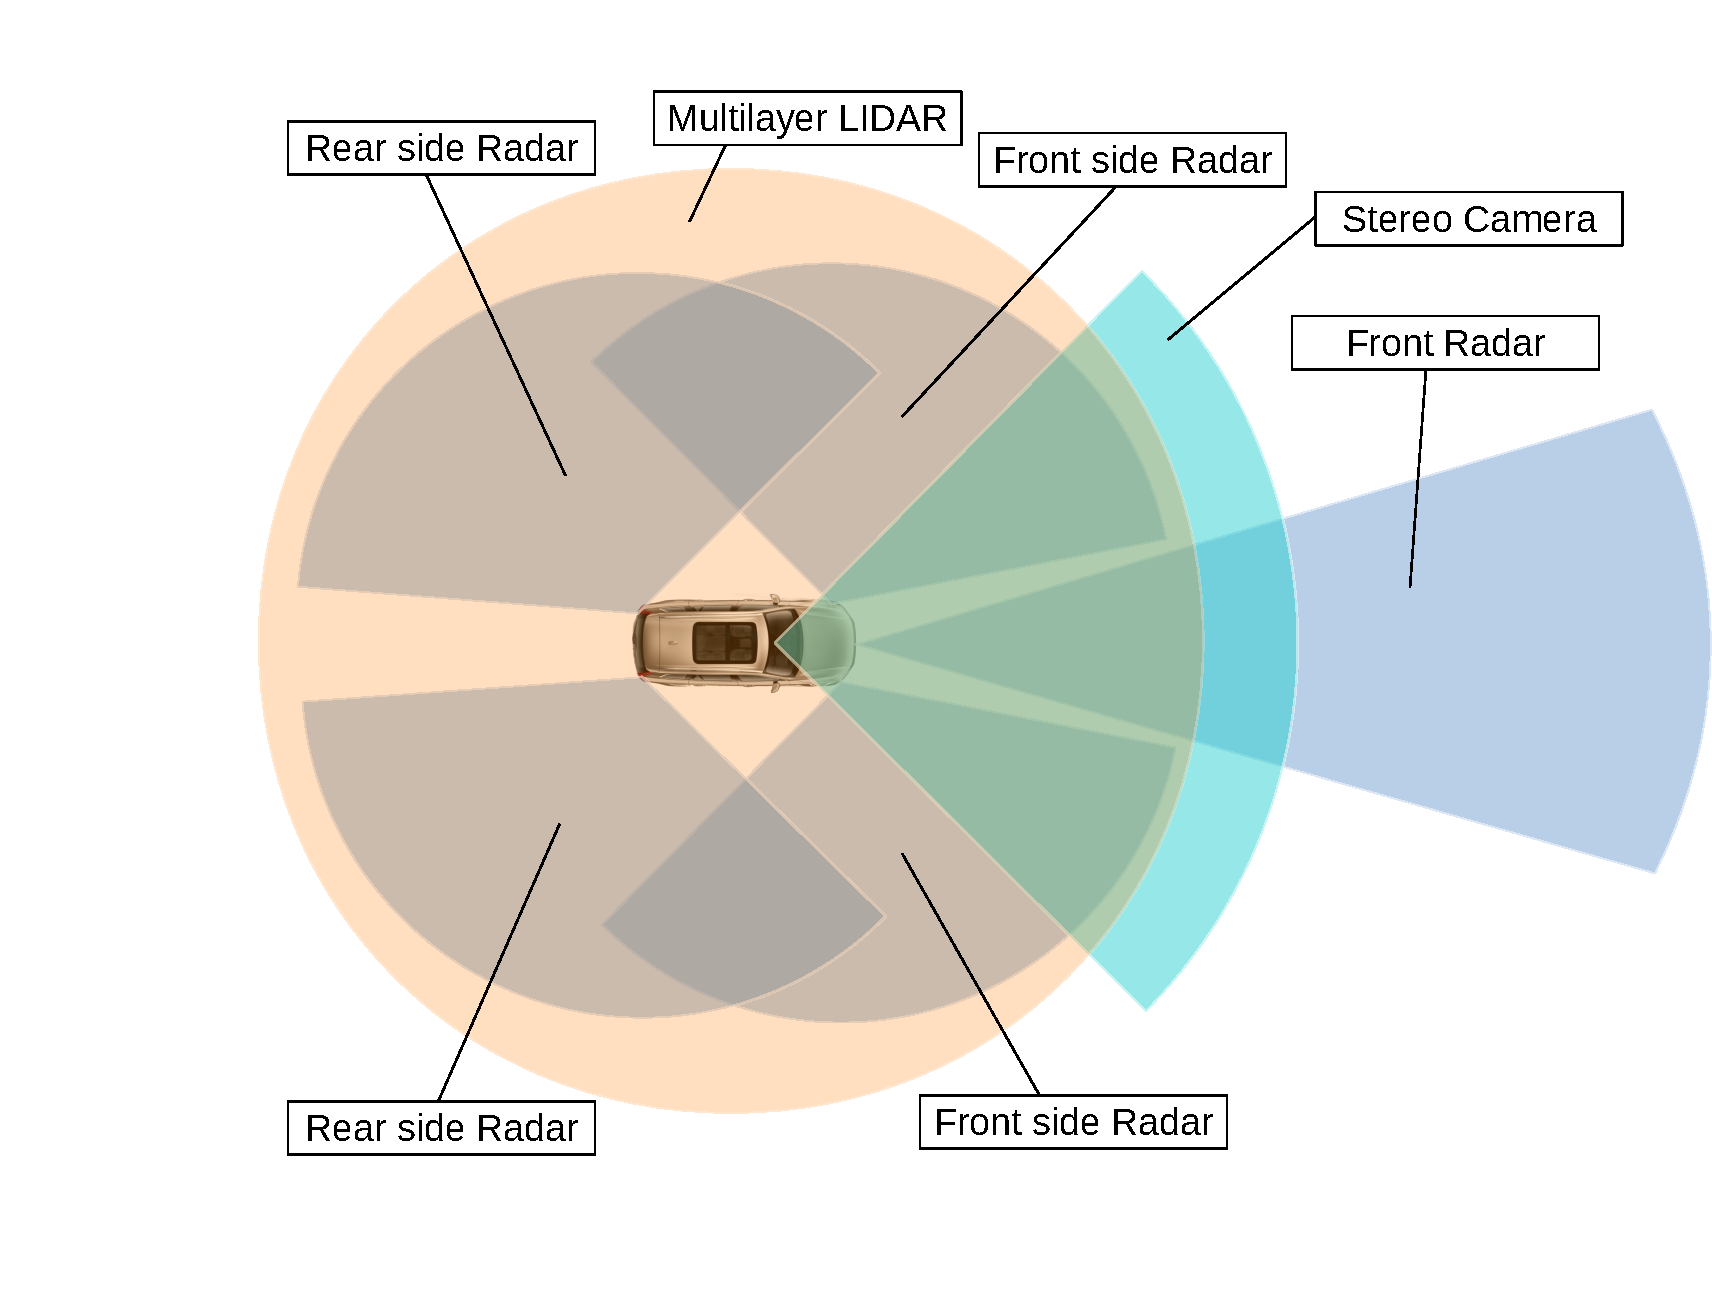
\includegraphics[width=\columnwidth]{sensors.pdf}
\label{platform}
%\end{center}
\end{figure}


Zusätlich zur Fahrzeuginternen Sensorik (Odometer, Interialsensorik) ist im Fahrzeug ein Applanix POS LV verbaut. Zu Zeitpunkt des Verfassens dieser Arbeit war es leider nicht möglich auf
die Radarsensoren und die Stereokamera zuzugreifen. Daher werden im folgenden lediglich der Velodyne Lidar und das Applanix System genauer beschrieben.

\subsection{Velodyne VLP-16 LiDAR}
Der Velodyne VLP-16 ist ein 360 Grad 3D Laserscannermit einer Rotationsgeschwindigkeit von 5 bis 20 Umdrehungen pro Sekunde. Er bietet ein vertikales FOV von 30 Grad, bei 2 Grad Auflösung.
Mit einer Reichweite von 100m kann er einen Umkreis von 200m Durchmesser abdecken. Weiterhin kann der VLP-16 mit dem Applanix POS LV syncronisiert werden, was eine jitterarme Zeimessung ermöglicht.
Eine weiter Funktion des Velodyne Sensors, ist das er auf verschiedene Messimpulse reagieren kann. Durch die Auswertung des letzten Impulses statt des Stärksten Impulses ist es Möglich durch Transparent Objekte zu sehen.
Das ermöglicht uns im späteren Verlauf die Breite des Fahrzeues zu ermitteln, da der Velodyne durch die Glasfenster des Fahrzeues blicken kann.
Bei einer eingestellten Geschwindigkeit von 10Hz liefert der VLP-16 eine Auflösung von 0.2 Grad bei einer Abreichung von +-3cm. Der VLP-16 ist mittig auf dem Dach des XC90 moniert, um eine möglichst hohe Positionierung
zu erreichen, die eine Rundumsicht umd Das Fahrzeug zu erreichen. Zu beachten ist, das diese Ausrichtung für den Sensor denkbar ungünstig ist, da der Sensor ein vertikales
Sichtfeld von -15 bis +15 Grad hat. Dadurch sind nachezu alle messungen über Null grad quasi nutzlos. Der blick auf die Herstellerseite
\footnote{\url{http://velodynelidar.com/vlp-16.html} (03/09/2017)}
verrät, das Der VLP-16 aunteranderem auf die verwendung mit Drohnen hin konstuiert wurde, während der Größere HDL64E
\footnote{\url{http://velodynelidar.com/hdl-64e.html} (03/09/2017)}
explizit für den Urbanen Automotivebereich beworben wird, und über ein Sichtfeld von +2 bis -24.9 Grad verfügt. Die dabei entstehenden Probleme werden später diskutiert.



\subsection{Applanix POS LV}
Das POS LV ist ein kompaktes Positions- und Orientierungssystem. Es Offeriert stabile, zuverlässige und reproduzierbare Positionierungslösungen für landgestützte Fahrzeuganwendungen.
Das POS LV liefert dabei eine Inertialsensork und Odometrie gestützte Positionsmessung mit einer Genauigkeit von bis zu 0.3m (bis zu 0.035m bei verwendung von der der RTK - Korrektur).
Im weiteren Verlauf wird außerdem das vom POS LV gelieferte Heading genutzt, welches eine Genauigkeit von 0.2 Grad liefert. Auch nach ausfall des GPS-Signals kann das POS-LV durch sein
Odeomerter und der Inertialsensork eine Position liefern. Diese wird jedoch über die Zeit schlechter, so das 60Sek nach Ausfall des GPS-Signals nich eine Genauigkeit von 2.51m erwartet
werden kann.\cite{manAP}






